%% cleanthesis-doc.tex
%% Copyright 2016 R. Langner
%
% This work may be distributed and/or modified under the
% conditions of the LaTeX Project Public License, either version 1.3
% of this license or (at your option) any later version.
% The latest version of this license is in
%   http://www.latex-project.org/lppl.txt
% and version 1.3 or later is part of all distributions of LaTeX
% version 2005/12/01 or later.
%
% This work has the LPPL maintenance status `maintained'.
%
% The Current Maintainer of this work is R. Langner.
%
% This work consists of all files listed in MANIFEST.md.
%
\documentclass{ltxdockit}
\usepackage{btxdockit}
\usepackage[utf8]{inputenc}
\usepackage[american]{babel}
\usepackage[strict]{csquotes}
\usepackage{tabularx}
\usepackage{longtable}
\usepackage{booktabs}
\usepackage{shortvrb}
\usepackage{pifont}
\usepackage{graphicx}

\rcsid{$Id: cleanthesis.tex,v 0.3.1 2015/08/26 23:32:00 derric stable $}

\newcommand*{\cleanthesis}{\emph{Clean Thesis}\xspace}
\newcommand*{\cthesishome}{http://cleanthesis.der-ric.de/}
%\newcommand*{\cthesisctan}{http://www.ctan.org/tex-archive/macros/latex/contrib/../}

\titlepage{%
  title={The \sty{cleanthesis} Package},
  subtitle={A Clean LaTeX Style for Thesis Documents},
  url={\cthesishome},
  author={Ricardo Langner},
  email={info@cleanthesis.der-ric.de},
  revision={\rcsrevision},
  date={\rcstoday}}

\hypersetup{%
  pdftitle={The \cleanthesis Package},
  pdfsubject={A Clean LaTeX Style for Thesis Documents},
  pdfauthor={Ricardo Langner},
  pdfkeywords={tex, latex, thesis, style}}


%\setcounter{secnumdepth}{4}

\begin{document}

\printtitlepage
\tableofcontents
%\listoftables

\section{Introduction}
\label{sec:intro}

\subsection[About]{About \sty{cleanthesis}}
\label{sec:intro:about}

\subsection{Donation}
\label{sec:intro:donation}

If you like the \cleanthesis style, or you have used it for one of your own documents successfully there are (at least) three different but pretty easy ways of saying thank you.

\paragraph{Report on issues and missing features} If you have ideas for new features, suggestions for improvements or you encounter problems and errors using the \cleanthesis style please report them using the issue tracker\footnote{\url{https://github.com/derric/cleanthesis/issues}} at the GitHub Project\footnote{\url{https://github.com/derric/cleanthesis}} or send an email to \texttt{issue[at]cleanthesis.der-ric.de}.

\paragraph{Be Social} I would very much appreciate a donation in the form of a blog post, tweet, or facebook post. Share your experience and your opinion. Talk to your friends, fellow students, or colleagues about the \cleanthesis style.

\paragraph{Send me a postcard} Based on the idea of André Miede: I would be very pleased about a donation in the form of a POSTCARD. You can find my address below this paragraph. I am going to collect all postcards and exhibit them on the website \url{\cthesishome}. My address is


\begin{itemize}
\item \textbf{Ricardo Langner} \\
Alfred-Schrapel-Str. 7 \\
01307 Dresden, Germany
\end{itemize}

\subsection{License}
\label{sec:intro:license}

Copyright \textcopyright\ 2016 R. Langner

This work may be distributed and/or modified under the
conditions of the LaTeX Project Public License, either version 1.3
of this license or (at your option) any later version.
The latest version of this license is in
  \url{http://www.latex-project.org/lppl.txt}
and version 1.3 or later is part of all distributions of LaTeX
version 2005/12/01 or later.

This work has the LPPL maintenance status `maintained'.

The Current Maintainer of this work is R. Langner.

This work consists of all files listed in MANIFEST.md.

\subsection{Feedback}
\label{sec:intro:feedback}

\subsection{Acknowledgments}
\label{sec:intro:ack}

First of all I would like to thank André Miede. He is the author of the Classic Thesis style. His Classic Thesis style inspired end encouraged me to publish my own thesis style. Thank you André for doing a great job.

I would like to thank the following people for using the \cleanthesis style and giving important initial feedback to me, e.g., features, bugs: (1) \textbf{Sebastian Kleinau}\footnote{\url{http://www.sk-downloading.de/} (in German only)} in his bachelor thesis, (2) \textbf{Mathias Frisch}\footnote{\url{http://wwwpub.zih.tu-dresden.de/~frisch/}} in his dissertation (PhD), and (3) \textbf{Anton Augsburg}\footnote{\url{http://antonaugsburg.de/} (in German only)} in his project thesis.

\subsection{Prerequisites}
\label{sec:intro:pre}

The following section gives an overview of all resources required by this package.

\subsubsection{Requirements}
\label{sec:intro:req}

\section{User Guide}
\label{sec:userguide}

\subsection{Package Options}
\label{sec:userguide:pkgopt}

All package options are given in \keyval notation.
The value \texttt{true} can be omitted for all boolean keys, \eg \opt{sansserif} without a value is equivalent to \kvopt{sansserif}{true}.

All of the following options must be used as \sty{cthesis} is loaded, \ie in the optional argument to \cmd{usepackage}.

\begin{optionlist}

\boolitem[false]{sansserif}

Sets whether to use a sans serif font or not.

\boolitem[false]{hangfigurecaption}

Sets whether to use a hanging figure label (similar to headlines, placed in page margin) or not.

\boolitem[true]{hangsection}

Sets whether to use a hanging section label (placed in page margin) or not.

\boolitem[true]{hangsubsection}

Sets whether to use a hanging sub-section label (placed in page margin) or not.

\optitem[endash]{figuresep}{\opt{none},\opt{colon},\opt{period},\opt{space},\opt{quad},\opt{endash}}

This option can be used to define a different label separator for cations of figures. The following value are allowed:

\begin{valuelist}
\item[none] Inserts no character in between.
\item[colon] Inserts a colon (\textbf{:}) in between.
\item[period] Inserts a period (\textbf{.}) in between.
\item[space] Inserts a single space character in between.
\item[quad] Inserts a \cmd{\\quad} in between.
\item[endash] Inserts an en dash (\textbf{--}) in between.
\end{valuelist}

\optitem[full]{colorize}{\opt{full},\opt{reduced},\opt{bw}}

This option can be used to define a color mode, i.e., what elements or parts of the document should be colored.
This allows you to reduce costs, if you need to print the document.
The following values are allowed:

\begin{valuelist}
\item[full] In this mode, almost every page uses some color, because the thin line besides the page number (footer) is colored.
	The following elements are colored as well: title of the document (title page), number of the chapter on the chapter page, name of the chapter in the footer, section and sub-section headlines, and figure labels.
\item[reduced] This mode reduces the use of colors to reasonable level.
	Footers are totally free of colors.
	Only the title page, chapter pages, section headlines, and figure labels are colored.
\item[bw] This mode completely eliminates all colors of the document style---every element is black or gray.
	If you do not use colored images either, the document is completely achromatic.
\end{valuelist}

\optitem[bluemagenta]{colortheme}{\opt{bluemagenta},\opt{bluegreen}}

This option can be used, to switch between different color presets.
These presets are used to colorize, e.g., headlines, footnotes, or chapter numbers.
This option has a reduced or no effect depending on the package option \texttt{colorize} (see above).
The following values are allowed:

\begin{valuelist}
\item[bluemagenta] Headlines and titles use a blue color, figure labels use magenta.
\item[bluegreen] Headlines and titles use a blue color, figure labels use green.
\end{valuelist}

\optitem[bibtex]{bibsys}{\opt{biber},\opt{bibtex}}

Sets whether to use \texttt{biber} or \texttt{bibtex} as citation management tool (engine).
The default (still) is \texttt{bibtex}.

"\texttt{Biber} [is] a BibTeX replacement for users of BibLaTeX", see \url{http://biblatex-biber.sourceforge.net/}.

\optitem[bib-refs]{bibfile}{file name of your bibtex file}

Sets the file name of the bibtex file used for the bibliography.
If this option is not used (defined), the package looks for the default bibliography \texttt{bib-refs.bib}.

\optitem[alphabetic]{bibstyle}{\opt{alphabetic},\opt{numeric},\opt{authoryear}}

Sets whether to use an \texttt{alphabetic}, a \texttt{numeric}, or an \texttt{authoryear} reference style for the bibliography.
For further information please check out the biblatex documentation\footnote{\url{http://www.ctan.org/pkg/biblatex}}.
The default is \texttt{alphabetic}.

\begin{figure}[th!]
	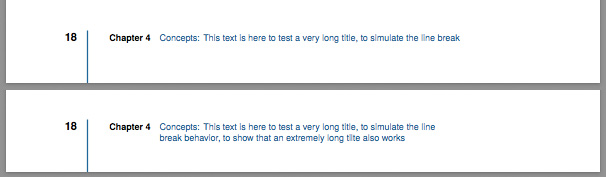
\includegraphics[width=\textwidth]{wrapfooter}
	\caption{The package option \texttt{wrapfooter} can be used to wrap very long chapter titles in the footer.}\label{fig:wrapfooter}
\end{figure}

\boolitem[false]{wrapfooter}

Sets whether to wrap the name of a chapter in the footer or not (Figure \ref{fig:wrapfooter}).

\end{optionlist}

\end{document}
